\begin{figure}
  \begin{center}
    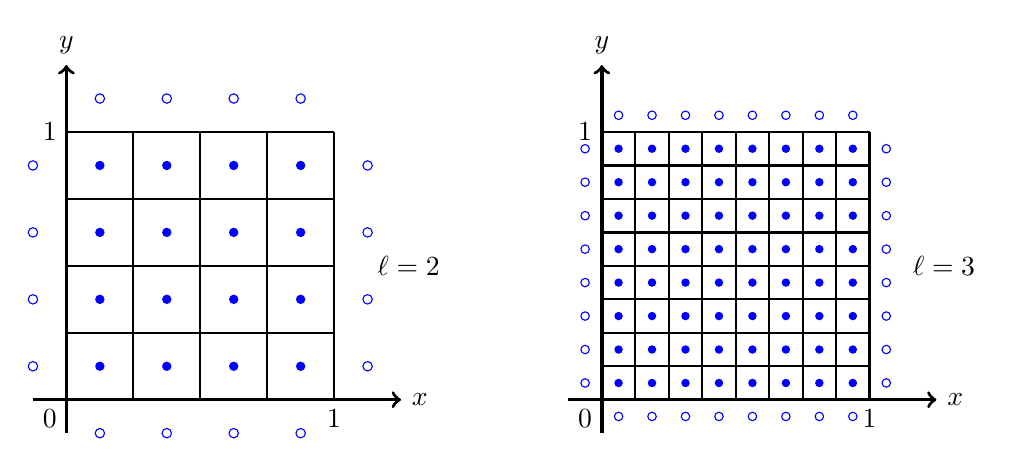
\begin{tikzpicture}[scale=0.85]
      % First grid (l=2)
      \begin{scope}
        % Grid lines
        \draw[thick] (0,0) grid (4,4);

        % Add axis labels for x=1 and y=1
        \node[black, below] at (4,0) {$1$};
        \node[black, left] at (0,4) {$1$};
        \node[black, below left] at (0,0) {$0$};

        % Axes
        \draw[black,->,very thick] (-0.5,0) -- (5,0) node[right] {$x$};
        \draw[black,->,very thick] (0,-0.5) -- (0,5) node[above] {$y$};

        % Grid points
        \foreach \x in {0.5,...,3.5} {
          \draw[blue] (\x,-0.5) circle (2pt);
          \draw[blue] (-0.5,\x) circle (2pt);
          \draw[blue] (\x,4.5) circle (2pt);
          \draw[blue] (4.5, \x) circle (2pt);
          \foreach \y in {0.5,...,3.5} {
            \fill[blue] (\x,\y) circle (2pt);
          }
        }


        % Level label
        \node[right] at (4.5,2) {$\ell=2$};
      \end{scope}

      % Second grid (l=3)
      \begin{scope}[xshift=8cm]
        % Grid lines
        \draw[thick, step = 0.5] (0,0) grid (4,4);

        % Add axis labels for x=1 and y=1
        \node[black, below] at (4,0) {$1$};
        \node[black, left] at (0,4) {$1$};
        \node[black, below left] at (0,0) {$0$};

        % Axes
        \draw[black, ->,very thick] (-0.5,0) -- (5,0) node[right] {$x$};
        \draw[black, ->,very thick] (0,-0.5) -- (0,5) node[above] {$y$};

%         % Grid points
        \foreach \x in {0.25,0.75,...,3.75} {
          \draw[blue] (\x,-0.25) circle (1.8pt);
          \draw[blue] (-0.25,\x) circle (1.8pt);
          \draw[blue] (\x,4.25) circle (1.8pt);
          \draw[blue] (4.25, \x) circle (1.8pt);
% 
          \foreach \y in {0.25,0.75,...,3.75} {
            \fill[blue] (\x,\y) circle (1.8pt);
          }
        }


        % Level label
        \node[right] at (4.5,2) {$\ell=3$};
      \end{scope}
    \end{tikzpicture}
  \end{center}
  \caption[Two-dimensional cell-centered grids and grid points.]{Example of two-dimensional cell-centered grids and grid points for $\ell=2$ and $\ell=3$. The ghost points are indicated by unfilled circles.}
\label{fig:2DCCgrid-example}
\end{figure}
